\documentclass{letter}
\usepackage[margin=0pt,a5paper]{geometry} % a5 is 148mm x 210mm
\usepackage{tikz}

\begin{document}
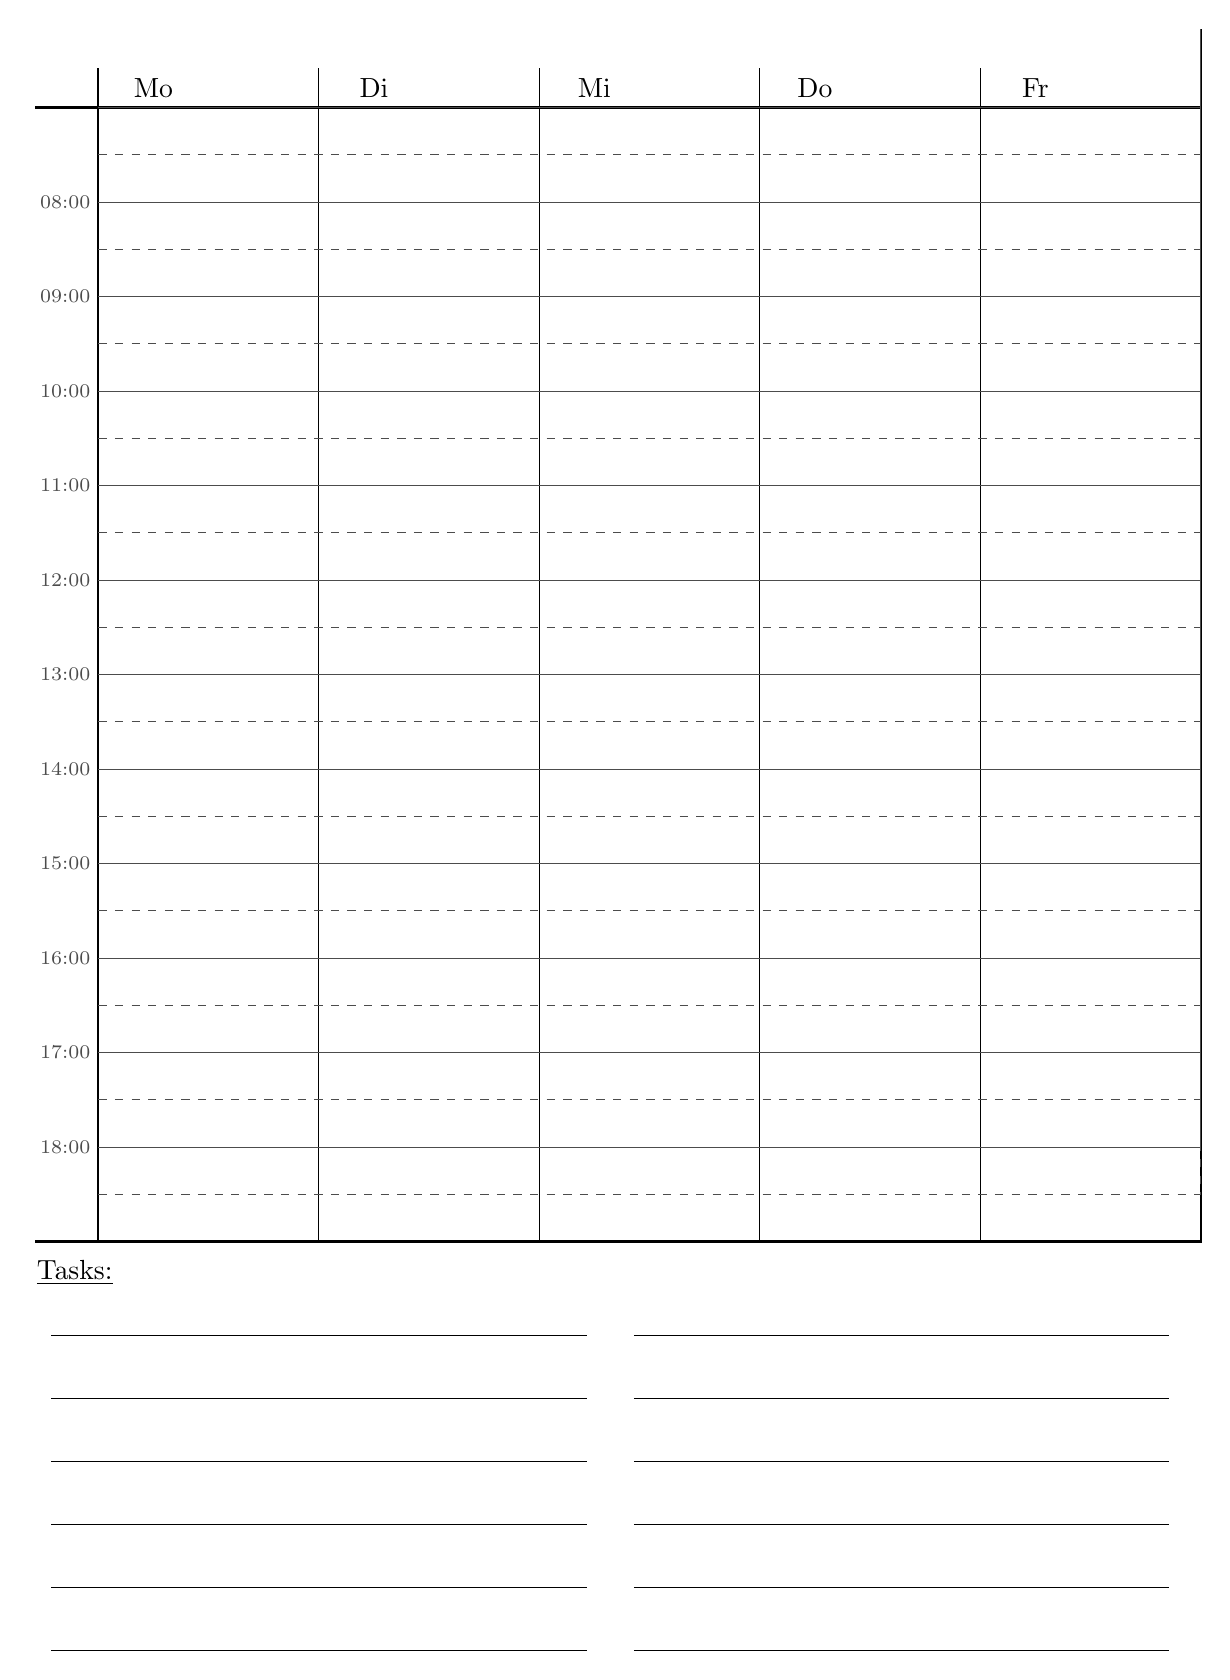
\begin{tikzpicture}
	\draw (0,0) coordinate;

	\begin{scope} % organizer
		\providecommand{\yspace}{1.2}
		\providecommand{\xspace}{2.8}
		\providecommand{\yend}{-1-12*\yspace}

		\begin{scope}[thick]
			\draw (0.8,-0.5) -- (0.8,\yend);
			\draw (0,-1) -- ++(14.8,0);
			\draw (0,\yend) -| (148mm,0);
		\end{scope}

		\begin{scope}[xshift=8mm] % days
			\foreach \x/\day in {1/Mo,2/Di,3/Mi,4/Do,5/Fr}
				{
					\draw (\x*\xspace,-0.5) -- (\x*\xspace,\yend);
					\draw (\x*\xspace - 0.75*\xspace, -0.75) node {\day};
				}
		\end{scope}

		% python: [(f"{i}/{7+i:02}:00") for i in range(1,12)]
		\begin{scope}[very thin,black!70] % times
			\foreach \y/\time in {0/,1/08:00,2/09:00,3/10:00,4/11:00,5/12:00,6/13:00,7/14:00,8/15:00,9/16:00,10/17:00,11/18:00}
				{
					\draw (0.8, -1-\y*\yspace) node[anchor=east,outer sep=0,inner sep=0,left=1mm] {\scriptsize \time} -| (148mm,0);
					\draw[dashed] (0.8, -1-\y*\yspace-0.5*\yspace) -| (148mm,0);
				}
		\end{scope}
	\end{scope}

	\begin{scope}[yshift=-15.8cm] % Tasks
	\draw (0.5,0) node {\underline{Tasks:}};

	\providecommand{\yspace}{0.8}
	\foreach \y in {1, ..., 6}{
	\draw (2mm,-\y*\yspace) -- (70mm,-\y*\yspace);
	\draw (76mm,-\y*\yspace) -- (144mm,-\y*\yspace);
	}
	\end{scope}
\end{tikzpicture}
\end{document}
